\section{Inštalácia operačného systému}
\paragraph{}
Ako serverový aj klientský operačný systém sme použili linuxovú distribúciu \say{Debian 8.6.0 x64 - kódové meno \say{Jessie} }Najprv sme si stiahli inštalačný iso súbor s \say{Debian 8.6.0 stable 64 bit} vo verzií \say{netinst} t.j. operačný systém si sťahuje aktuálne balíčky z internetu.
\paragraph{}
V rámci nastavení počítačov (serverov a desktopov) vo VirtualBox-e sme zmenili tieto nastavenia:
\begin{itemize}
\item System -\textgreater{} Motherboard -\textgreater{} Base memory = 1024MB
\item System -\textgreater{} Processor -\textgreater{} Processor(s) = 1 CPU
\item System -\textgreater{} Processor -\textgreater{} Enable PAE/NX = zaškrtnúť
\item System -\textgreater{} Acceleration -\textgreater{} Hardware Virtualization -\textgreater{} Enable VT-x/AMD-V = zaškrtnúť
\item Storage -\textgreater{} Controller: IDE -\textgreater{} klikneme na Empty disk -\textgreater{} v pravom paneli klikneme na ikonku CD a vyberieme možnosť Choose Virtual Optical Disk File. Otvorí sa dialógové okno, v ktorom vyhľadáme stiahnutý iso súbor.
\item Pre servery a desktopy: Network -\textgreater{} Adapter 1 -\textgreater{} Enable Network Adapter a nastavíme Attached to -\textgreater{} Bridged Adapter -\textgreater{} eth1. Sieťové nastavenia pre firewall sú rovnaké, ako pre desktopy a servery, s tým, že Adapter 1 sme nastavili na Bridged Adapter pripojený na eth1 (lokálne rozhranie) a navyše sme zapli aj Adapter 2 ako Bridged Adapter pripojený na eth0 (verejné rozhranie).
\end{itemize}

\paragraph{}
Po nastavení virtuálky sme ju spustili. Ďalej sme postupovali v štandardnej inštalá\-cií Debian-u. Ako doménu sme nastavili takú, ktorá nám bola pridelená: \say{sos3.local}. Ako hostname sme nastavili doménové meno, ktoré je odvodené od jej funkcie napr. všetky servery majú označenie \say{SX} a desktopy \say{DX}, kde X je poradové číslo servera/desktopu. Z doplnkový balíškov sme pre servery neinštalovali nič, jedine pre desktopy sme nainštalovali grafické rozhranie XFCE.

\section{VLAN}
\paragraph{}
Servery sú vo VLAN 10, desktopy vo VLAN 20. Smerovanie medzi VLAN-ami je vykonávané na FW preto sme na firewall-e nainštalovali balíček \say{vlan}. Tento balíček pridá do systému softvérovú podporu podrozhraní, samotný sieťový adaptér podrozhrania podporoval. Prostredníctvom podrozhraní uskutočňujeme VLAN smerovanie, ktoré je bližšie popísané v kapitole \say{Firewall}.

\noindent
{\fontfamily{qcr}\selectfont
\begin{small}
\begin{verbatim}

apt-get install vlan

\end{verbatim}
\end{small}
}

\paragraph{}
Konfigurácia VLAN a trunking prebiehala na Cisco Catalyst prepínači. Servery S1 a S2 boli pripojené na rozhranie fa0/2 , firewall na fa0/3 a desktopy na fa0/1. Vytvorili sme VLANky a pomenovali ich. Nižšie uvádzame príkazy na konfiguráciu prepínača.


\noindent
{\fontfamily{qcr}\selectfont

% Urob text mensi, aby sa vosiel na sirku obrazovky
\begin{small}

% Pouzijeme "verbatim", aby sme escapeovali cely odsek
\begin{verbatim}

switch(config)# Vlan 10
switch(config-vlan)# name servers

switch(config)# Vlan 20
switch((config-vlan)# name PCs

switch(config)# interface fa0/3
switch(config-if)# switchport mode trunk
switch(config-if)# switchport trunk native vlan 1
switch(config-if)# no shut

switch(config)# interface fa0/2
switch(config-if)# switchport mode access 
switch(config-if)# switchport access vlan 10
switch(config-if)# no shut

switch(config)# interface fa0/1
switch(config-if)# switchport mode access 
switch(config-if)# switchport access vlan 20
switch(config-if)# no shut

\end{verbatim}
\end{small}
}

\section{Základná konfigurácia}
\paragraph{}
Každý inštalácia Debian-u obsahovala navyše tieto balíčky:

\noindent
{\fontfamily{qcr}\selectfont
\begin{small}
\begin{verbatim}

apt-get install tcpdump vim openssh-client openssh-server bind9-host

\end{verbatim}
\end{small}
}

\paragraph{}
Stručný popis balíčkov:

\begin{itemize}
\item tcpdump - nástroj na sledovanie sieťovej premávky
\item vim - textový editor
\item openssh-client / openssh-server - SSH kliet / server
\item bind9-host - nástroj na vykonávanie DNS dotazovania
\end{itemize}

\paragraph{}
Potom sme nainštalovali \say{VirtualBox Guest Additions}, pre zaistenie vyššej stability a kompatibility so zariadeniami a samotným virtualizovaným systémom.

\paragraph{}
Ďalej sme si nastavili statickú IP adresáciu na serveroch a firewall-e. Preto sme upravovali súbor \say{/etc/network/interfaces}. Nižšie je uvedený spomenutý konfiguračný súbor pre firewall.

\noindent
{\fontfamily{qcr}\selectfont

% Urob text mensi, aby sa vosiel na sirku obrazovky
\begin{small}

% Pouzijeme "verbatim", aby sme \say{escapeovali} cely odsek
\begin{verbatim}

source /etc/network/interfaces.d/*

# The loopback network interface
auto lo
iface lo inet loopback
# The primary network interface
allow-hotplug eth0
iface eth0 inet static
        address 158.193.139.74
        netmask 255.255.255.0
        gateway 158.193.139.1
        up /usr/local/etc/firewall.sh

auto eth0:1
allow-hotplug eth0:1
iface eth0:1 inet static
        address 158.193.139.75
        netmask 255.255.255.0
        gateway 158.193.139.1

# Vnutorna (firemna) sietovka
auto eth1

#VLAN 10 subinterface
auto eth1.10
iface eth1.10 inet static
        address 192.168.0.1
        netmask 255.255.255.128
        dns-nameservers 192.168.0.2 192.168.0.3

#VLAN 20 subinterface
auto eth1.20
iface eth1.20 inet static
        address 192.168.0.129
        netmask 255.255.255.128
        dns-nameservers 192.168.0.2 192.168.0.3

# This is an autoconfigured IPv6 interface
iface eth0 inet6 auto

\end{verbatim}
\end{small}
}



\section{DNS}
\paragraph{}
Systém názvov domén alebo systém mien domén, alebo systém doménových mien (Domain Name System), skr. DNS, je systém, ktorý ukladá prístup k informácii o názve zariadení (hostname) a názve domény v istej distribuovanej databáze v počítačových sieťach ako internet. Najdôležitejšie je, že poskytuje mechanizmus získania IP adresy pre každé doménové meno zariadenia (lookup) a naopak (reverse). Uvádza aj záznamy pre poštové servery (MX záznam) akceptujúce poštu pre danú doménu.
\paragraph{}
DNS poskytuje na internete všeobecne dôležitú službu, pretože kým počítače a sieťový hardvér pracujú s IP adresami, ľudia si vo všeobecnosti ľahšie pamätajú mená strojov a domén pri použití napr. v URL a e-mailovej adrese (obzvlášť nepríjem\-né by to bolo pri IPv6 adrese). DNS tak tvorí prostredníka medzi potrebami človeka a softvéru.
\paragraph{}
V rámci našej doménovej zóny \say{sos3.local} sme si museli nastaviť dva DNS servery: Master (S1) a Slave (S2). Slave zrkadlí hlavný DNS server a v prípade poruchy ho zastúpi. Keďže si Slave DNS server všetko stiahne z Master DNS servera, netreba ho primárne konfigurovať, ale stačí mu  nastaviť \say{allow-transfer} na privátnu IP Master DNS.
\paragraph{}
Na obidva servery sme nainštalovali DNS server a nástroje na overenie jeho funkčnosti:

\noindent
{\fontfamily{qcr}\selectfont
\begin{small}
\begin{verbatim}

apt-get install bind9 bind9utils dnsutils

\end{verbatim}
\end{small}
}


\paragraph{}
Master DNS serveru sme upravovali súbory \say{/etc/resolv.conf}, kvôli konfigurácií adries DNS serverov, \say{/etc/bind/master/db.sos3.local} (view-lokálny),\\ \say{/etc/bind/master/db.sos3.external} (view-verejný), \say{/etc/bind/named.conf.local} (definovanie lokálnych a verejných DNS pohľadov). Pohľady na DNS serveri sme definovali kvôli tomu, aby sme vedeli dať tomu, kto sa pýta, správnu IP adresu v závislosti od toho, odkiaľ sa pýta. Pokiaľ sa dotazuje klient z lokálnej siete, DNS server mu odpovie IP adresou v lokálnej sieti. Pokiaľ sa ale pýta klient z vonkajšej siete (internetu), DNS server odošle klientovi verejnú IP adresu. Obsah súboru \say{/etc/resolv.conf} je uvedený nižšie.

\noindent
{\fontfamily{qcr}\selectfont

% Urob text mensi, aby sa vosiel na sirku obrazovky
\begin{small}

% Pouzijeme "verbatim", aby sme escapeovali cely odsek
\begin{verbatim}

domain sos3.local
# Master DNS
nameserver 192.168.0.2
# Slave DNS
nameserver 192.168.0.3

\end{verbatim}

\end{small}

}

\paragraph{}
V adresári \say{/etc/bind} na S1 sme vytvorili adresár \say{master}, do ktorého sme ukladali zónové súbory pre DNS.
\paragraph{}
Pohľady pre DNS sme nastavovali na Master DNS serveri súbormi\\ \say{/etc/bind/named.conf.local} (obr. \ref{fig:dns_views}), \say{/etc/bind/master/db.sos3.local} (obr. \ref{fig:dns_internal}),\\ \say{/etc/bind/master/db.sos3.external} \ref{fig:dns_external}). Pri dotazovaní na doménové meno nášho DNS zvnútra sa použijú privátne adersy DNS serverov zo súboru\\ \say{/etc/bind/master/db.sos3.local}. Pri dotazovaní na doménové meno nášho DNS zvonku sa použijú verejné adersy DNS serverov zo súboru\\ \say{/etc/bind/master/db.sos3.external}. O tom, aký súbor (pohľad) sa použije, rozhoduje súbor \say{/etc/bind/named.conf.local}
\paragraph{}
S počítačmi v lokálnej sieti vieme komunikovať pomocou ich doménových mien (napr. ping). Docielili sme to úpravou lokálneho pohľadu (viď obr. \ref{fig:dns_internal})Preklad doménových mien na IP adresy je definovaný v súbore\\ \say{/etc/bind/master/db.sos3.local}.
\paragraph{}
V súbore \say{/etc/bind/named.conf.options} sme nastavili adresu preposielacieho DNS servera. Preposielací DNS server (tiež známy ako \say{DNS forwarder}) sa použije vtedy, ak lokálne DNS servery nemajú požadovaný záznam. Lokálny DNS server v takom prípade kontaktuje preposielací DNS server, ktorý dotazované doménové meno preloží za nás.
\paragraph{}
Firewall bol nakonfigurovaný tak, aby prepúšťal DNS požiadavky na lokálnej sieti, a tiež aby prepúšťal požiadavky z internetu na obidva DNS servery t.j. aby boli obidva DNS servery viditeľné zvonku (PREROUTING). Záznamy pre DNS sú pre obidve verejné IP adresy pre udp aj tcp port 53 (zdrojový aj cieľový).
\paragraph{}
V prípade, že sa vyskytli problémy, skúšali sme vypnúť firewall, kontrolovali sme konfiguračné súbory Master DNS servera príkazmi \say{named-checkconf} a \say{named-checkzone} a príkazom \say{tcpdump} sme monitorovali prenášané správy. Pri každej zmene konfiguračných súborov bolo treba reštartovať službu \say{bind9}.

\paragraph{}
Výnimky pre DNS vo firewall-e sú uvedené v kapitole \say{Firewall}.

\paragraph{}
TODO - chyba vam aj overenie master/sôave klucmi, to nemate vobec popsaine
TODO - Toto netsaci, viwes mali byt vsade aj pre default zony, dorrobit
\\
\\
\noindent
Zdroje:\\
\noindent
https://www.howtoforge.com/two\_in\_one\_dns\_bind9\_views\\

\begin{figure}[!htb]
\centering
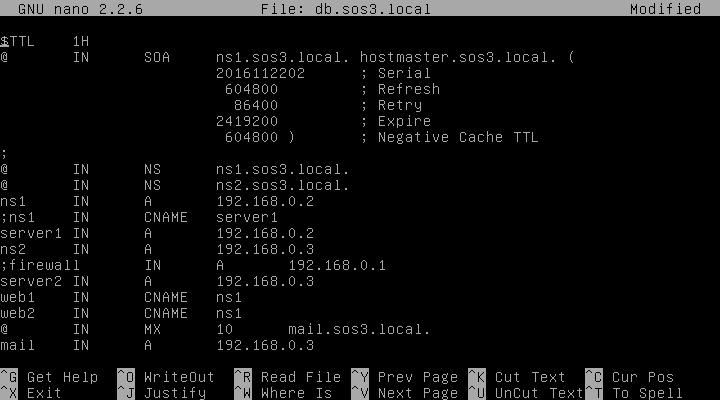
\includegraphics[scale=0.79]{linux_master_local}
\caption{Vnútorné DNS záznamy}
\label{fig:dns_internal}
\end{figure}

\begin{figure}[!htb]
\centering
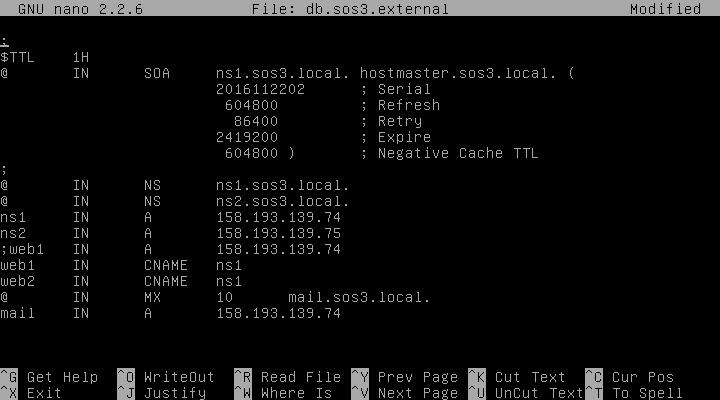
\includegraphics[scale=0.79]{linux_master_external}
\caption{Verejné DNS záznamy}
\label{fig:dns_external}
\end{figure}

\begin{figure}[!htb]
\centering
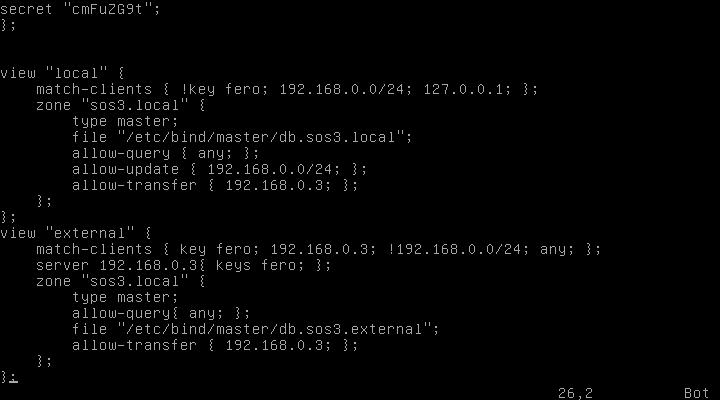
\includegraphics[scale=0.79]{linux_dns_views}
\caption{Nastavenie parametrov pre DNS pohľady a autentifikácia Slave DNS servera spoločným kľúčom}
\label{fig:dns_views}
\end{figure}

\begin{figure}[!htb]
\centering
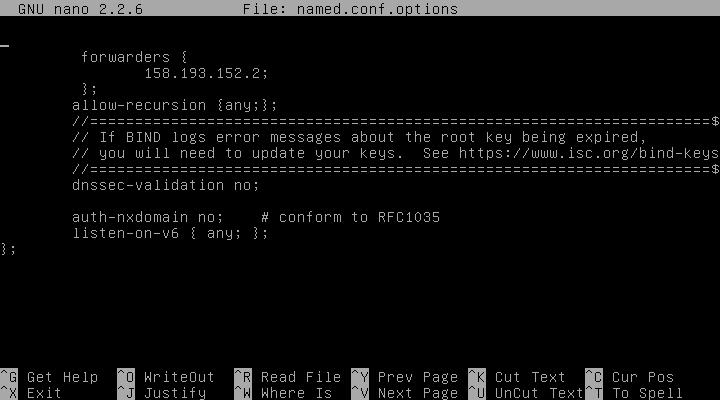
\includegraphics[scale=0.79]{linux_named_options}
\caption{Konfigurácia DNS forwardera}
\label{fig:dns_forwarder}
\end{figure}


\section{DHCP}
\paragraph{}
Dynamic Host Configuration Protocol (DHCP) je súbor zásad, ktoré využívajú komunikačné zariadenia (počítač, router alebo sieťový adaptér), umožňujúci zariadeniu vyžiadať si a získať IP adresu od servera, ktorý má zoznam adries voľných na použitie.DHCP Server (Dynamic Host Configuration Protocol) vykonáva automatické pridelenie IP adries svojim klientom. Môžu to byť akékoľvek systémy, podporujúce DHCP. DHCP je štandardný protokol, môžu ho využívať aj systémy mimo Microsoft. Z Microsoft operačných systémov podporujú funkciu DHCP klienta všetky až na veľmi exotický LAN Manager pre OS / 2. V rámci siete potom máme DHCP Server - prideľujúca adresy a počítače - ktoré je od neho preberajú (DHCP Clients). V sieti môžu byť aj počítače, ktoré majú tieto adresy nastavené manuálne.

\paragraph{}
DHCP server (S2) sme museli upraviť tak, aby prideľoval aj DNS adresy serverov. Súbor \say{/etc/dhcp/dhcpd.conf} na S1 sme upravili tak, že sme doň pridali privátne IP adresy DNS serverov (option domain-name-servers). Do časti pre podsieť sme definovali názvy týchto serverov. Voľbu \say{optionhost-name} sme zmenili z pôvodného \say{example.org} na \say{sos3.local}. Tým, že sme nastavili DNS server, nemusíme meniť na jednotlivých hostoch súbor \say{/etc/resolv.conf}.
Preto sme na FW museli nainštalovať balíčky pre DHCP preposielací server a podporu VLAN

\noindent
{\fontfamily{qcr}\selectfont
\begin{small}
\begin{verbatim}

apt-get install isc-dhcp-server vlan

\end{verbatim}
\end{small}
}

\paragraph{}
Potom sme editovali súbor \say{/etc/network/interfaces} tak, že sme odstránili adresné informácie z vnútorného interfacu eth1, ale nechali sme \say{auto eth1}, aby sa port zapol (UP). Následne sme pridali subinterface eth1.10 pre VLAN 10 (servery) a eth1.20 pre VLAN 20 (desktopy). Adresný rozsah pre jednotlivé VLAN bola sieť 192.168.0.0/24 rozdelená na dve /25 siete: 192.168.0.0 - 192.168.0.127 pre VLAN 10 a 192.168.0.128 - 192.168.0.255 pre VLAN 20

\paragraph{}
FW plní úlohu DHCP Relay servera. Všetky DHCP požiadavky od klientov prechá\-dzajú cez FW ku DHCP serveru, ktorý pridelí klientovi IP adresu a ďalšie nakonfigurované informácie. Týmto spôsobom je FW zodpovedný iba za filtrovanie premávky a server za služby poskytované na sieti. IP adresa DHCP servera sa do konfiguračného súboru \say{/etc/default/isc-dhcp-relay} DHCP relay agenta musí zadať BEZ úvodzoviek a musíme počúvať na obidvoch podrozhraniach t.j. eth1.10 aj eth1.20. Konfigurácia DHCP Relay servera je uvedená nižšie.

\noindent
{\fontfamily{qcr}\selectfont

% Urob text mensi, aby sa vosiel na sirku obrazovky
\begin{small}

% Pouzijeme "verbatim", aby sme escapeovali cely odsek
\begin{verbatim}

# Defaults for isc-dhcp-relay initscript
# sourced by /etc/init.d/isc-dhcp-relay
# installed at /etc/default/isc-dhcp-relay by the maintainer scripts

#
# This is a POSIX shell fragment
#

# What servers should the DHCP relay forward requests to?
# Forwarduj DHCP poziadavky na S2
SERVERS=192.168.0.3

# On what interfaces should the DHCP relay (dhrelay) serve DHCP requests?
# Pocuvame DHCP REQUESTY na vlane 20 pre desktopy, ale aj na vlane 10, aby 
# sme mohli REQUEST poslat na server
INTERFACES="eth1.10 eth1.20"

# Additional options that are passed to the DHCP relay daemon?
OPTIONS=""

\end{verbatim}

\end{small}

}

\paragraph{}
Výnimky pre DHCP vo firewall-e sú uvedené v kapitole \say{Firewall}.

\paragraph{}
TODO - Konifg nie je vobec popisany---dorobit prerobit

\begin{figure}[!htb]
\centering
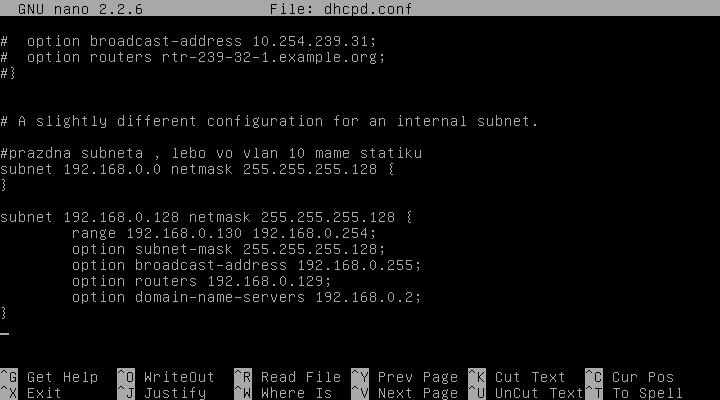
\includegraphics[scale=0.79]{linux_dhcp}
\caption{Konfiguračný súbor pre DHCP}
\label{fig:dhcp_config}
\end{figure}

\section{NTP}
\paragraph{}
NTP(Network Time Protocol) je protokol na sychronizáciu všetkých počítačov pripojených do vnutornej siete. Tento protokol zaisťuje, aby všetky počítače v sietei mali rovnaký a presný čas. Bol nvrhnutý aby odolával následkom premenlivého zdržania pri doručovaní paketov. NTP používa UDP na porte 123. NTP server sme zvolili server2, ktorý má ip adresu 192.168.0.3. Nainštalovali sme NTP príkazom

\noindent
{\fontfamily{qcr}\selectfont
\begin{small}
\begin{verbatim}

apt-get install ntp

\end{verbatim}
\end{small}
}


\paragraph{}
Na klientoch sme nainštalovali NTP pomocou príkazu


\noindent
{\fontfamily{qcr}\selectfont
\begin{small}
\begin{verbatim}

apt-get install ntp ntpdate

\end{verbatim}
\end{small}
}

\paragraph{}
V súbore na serveri s2 \say{/etc/ntp.conf} sme pridali slovenské servery zo stránky \say{www.pool.ntp.org/zone/sk}, ostatné servery sme zakomentovali. Klienti si následne z master serveru aktualizujú čas.
\paragraph{}
Výnimky pre NTP vo firewall-e sú uvedené v kapitole \say{Firewall}.

\paragraph{}
TODO - Konfig ntp klienta bol aky? Kto je ntp masdter pre firmu s2?

\begin{figure}[!htb]
\centering
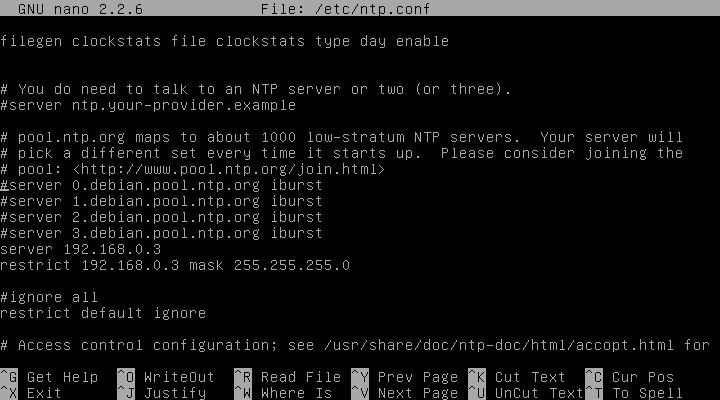
\includegraphics[scale=0.79]{linux_ntp_konfiguracia_server}
\caption{Konfigurácia NTP servera}
\label{fig:ntp_config_server}
\end{figure}

\begin{figure}[!htb]
\centering
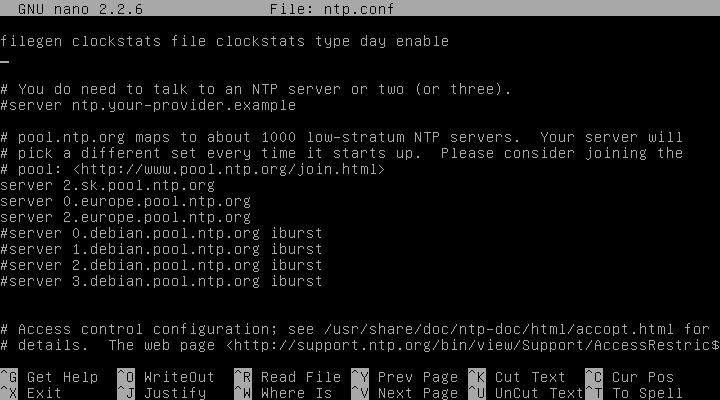
\includegraphics[scale=0.79]{linux_ntp_konfiguracia_klient}
\caption{Konfigurácia NTP na klientovi}
\label{fig:ntp_config_client}
\end{figure}

\begin{figure}[!htb]
\centering
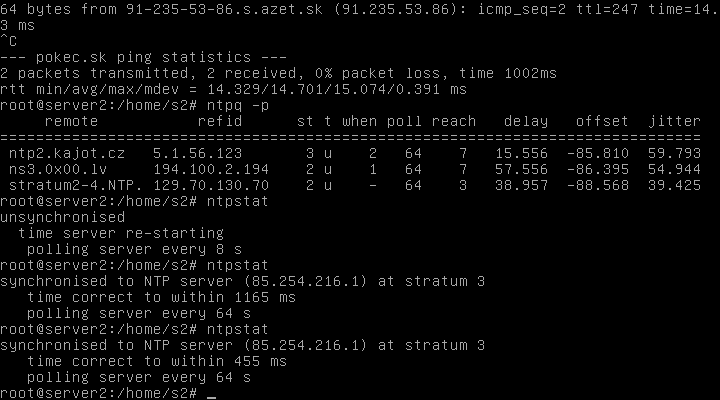
\includegraphics[scale=0.79]{linux_ntp_1}
\caption{Kontrola externých NTP serverov}
\label{fig:ntp_config_valid_1}
\end{figure}

\begin{figure}[!htb]
\centering
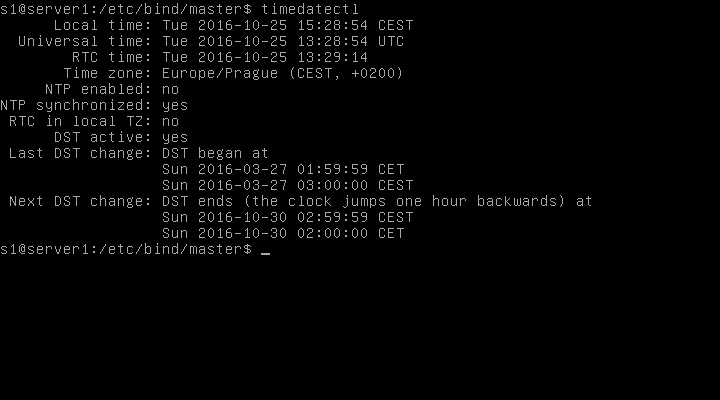
\includegraphics[scale=0.79]{linux_ntp_2}
\caption{Stav synchronizácie s NTP serverom}
\label{fig:ntp_config_valid_2}
\end{figure}

\section{Web server}
\paragraph{}
Apache HTTP Server je softwarový webový server s Opensource licenciou pre Linux, BSD, Microsoft Windows a iné platformy.
\paragraph{}
PHP (PHP: Hypertext Preprocessor) je populárny opensource skriptovací jazyk, ktorý sa používa najmä na programovanie klient-server aplikácií (na strane servera) a pre vývoj dynamických webových stránok.
\paragraph{}
MySQL je slobodný a otvorený viacvláknový, viacužívateľský SQL relačný databázový server. MySQL je podporovaný na viacerých platformách (ako Linux, Windows či Solaris) a je implementovaný vo viacerých programovacích jazykoch ako PHP, C++ či Perl. Databázový systém je relačný, typu DBMS (database management system). Každá databáza je v MySQL tvorená z jednej alebo z viacerých tabuliek, ktoré majú riadky a stĺpce. V riadkoch sa rozoznávajú jednotlivé záznamy, stĺpce udávajú dátový typ jednotlivých záznamov, pracuje sa s nimi ako s poľami. Práca s MySQL databázou je vykonávaná pomocou takzvaných dotazov, ktoré vychádzajú z programovacieho jazyka SQL (StructuredQueryLanguage).
\paragraph{}
Na webový server sme použili apache. Apache HTTP Server je softwarový webový server s Opensource licenciou pre Linux, BSD, Microsoft Windows a iné platformy. V dnešnej dobe je najrozšírenejším na celom svete. Pre plnú fukncionalitu webového servera sme museli nainštalovať apache, mysql, php príkazom

\noindent
{\fontfamily{qcr}\selectfont
\begin{small}
\begin{verbatim}

apt-get install apache2 mysql php5

\end{verbatim}
\end{small}
}

\paragraph{}
TODO - Akosa instaloval mysql..co sa pytal?

\paragraph{}
V adresári /var/www/ sme vytvorili priečinky s názvami web1 a web2. Kde web1 a web2 predstavovali dva virutálne webové servery. Následne sme v etc/apache2/sites-available 003-wiki.sos3.local.conf sme pridali cestu ku web stránke /var/www/web1 a ServerName web2.sos3.local. Pre joomlu v súbore 002-joomla.sos3.local.conf sme pridlai cestu k adresaru DocumentRoot /var/www/web1 a ServerName\\ web1.sos3.local . Následne do DNS záznamov sme museli pridať:	

\paragraph{}
pre súbor \say{db.sos1.local}

\noindent
{\fontfamily{qcr}\selectfont

% Urob text mensi, aby sa vosiel na sirku obrazovky
\begin{small}

% Pouzijeme "verbatim", aby sme escapeovali cely odsek
\begin{verbatim}

web1 IN A 192.168.0.4
web2 IN A 192.168.0.4


\end{verbatim}
\end{small}
}

\paragraph{}
a pre súbor \say{db.sos1.public}

\noindent
{\fontfamily{qcr}\selectfont
\begin{small}
\begin{verbatim}

web1 IN A 158.193.139.74
web2 IN A 158.193.139.74

\end{verbatim}
\end{small}
}


\paragraph{}
TODO - A2ensite chyba...t.j. sites-available je nanic bez sites-enabled


\subsection{Joomla}
\paragraph{}
V priečinku /var/www/web2 sme stiahli joomlu verziu 3.6 pomocou príkazu \say{wget https://github.com/.../Joomla\_3.6.0-Stable-Full\_Package.zip} . V ďalšom kroku sme odzipovali tento súbor príkazom \say{unzip Joomla\_3.6.0-Stable-Full\_Package.zip} . Nás\-ledne sme v prehliadači otvorili web1.sos3.local a podľa príslušných krokov sme nainštalovali joomlu.

\subsection{Mediawiki}
\paragraph{}
V priečinku var/www/web1 sme stiahli Wikimedia pomocou príkazu\\ \say{wget https://www.mediawiki.org/wiki/Download/mediawiki-1.2.8.zip} . Následne sme odzipovali tento súbor príkazom \say{unzip mediawiki-1.2.8.zip} . A v poslednom kroku sme v prehliadači web2.sos3.local nainštalovali mediawiki.

\paragraph{}
Výnimky pre webový server vo firewall-e sú uvedené v kapitole \say{Firewall}.

\begin{figure}[!htb]
\centering
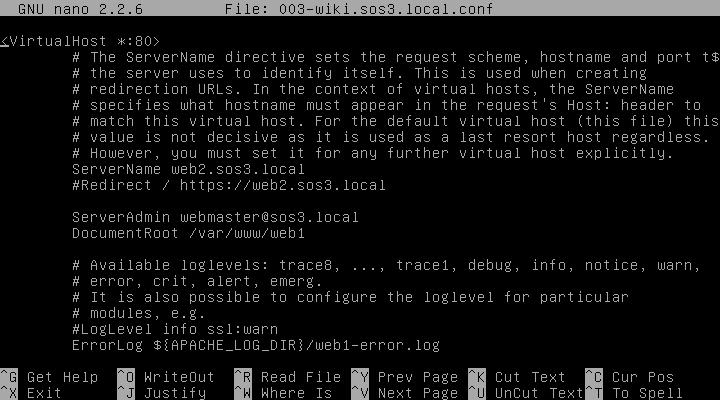
\includegraphics[scale=0.79]{linux_web1_konfiguracia}
\caption{Konfiguračný súbor webstránky}
\label{fig:web1_config_file}
\end{figure}

\begin{figure}[!htb]
\centering
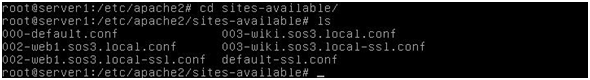
\includegraphics[scale=0.97]{linux_web_konfiguraky_webstranok}
\caption{Prehľad konfiguračných súborov webstránok}
\label{fig:web_config_files_list}
\end{figure}

\section{Poštový server}
\paragraph{}
Na poštový server sme použili postfix.Postfix je počítačový program pre unixové systémy pro prepravu elektronickej pošty (MTA).
\paragraph{}
Najprv bolo ptorebné nainštalovať postfix príkazom

\noindent
{\fontfamily{qcr}\selectfont
\begin{small}
\begin{verbatim}

apt-get install postfix

\end{verbatim}
\end{small}
}

\paragraph{}
Prešli sme inštaláciou kde sme nastavili hostname sos3.local. Následne sme museli reštar\-tovať postfixservicepostfixrestart. V súbore /etc/postfix/main.cf je potrebné upraviť myhostname = sos3.local, odkomentovať\\
\paragraph{}
TODO - pridat konfiguraky a obrazky
TODO - Toto nieje uplne ani zdaleka

\section{Firewall}
\paragraph{}
Politika filtrovania sieťovej premávky bola reštriktívna, t.j. čo nebolo vyslovene povolené, bolo zakázané. Pre filtrovanie sme použili nástroj \say{iptables}. Firewall sme konfigurovali priebežne s úlohami počas semestra. Skript bol uložený v\\ \say{/etc/skripty/firewall.sh}. Skriptu sme nastavili oprávnenia \say{chmod 744 firewall.sh}, aby ho mohol spúšťať iba root resp. sudo používateľ. Pravidlá v skripte sú štruktúro\-vané podľa protokolu resp. funkcie, ktorú vykonávajú. Nižšie je uvedený konfiguračný skript na pridávanie pravidiel pre iptables.

\noindent
{\fontfamily{qcr}\selectfont
\\

% Urob text mensi, aby sa vosiel na sirku obrazovky
\begin{small}

% Pouzijeme "verbatim", aby sme escapeovali cely odsek
\begin{verbatim}

#!/bin/bash

I=/sbin/iptables

# Vyčistíme pôvodné pravidlá z tabuliek NAT a FILTER
$I -F -t filter
$I -F -t nat

# Používame reštriktívnu politiku:
# čo nie je vyslovene povolené, je zakázané
$I -P INPUT DROP
$I -P FORWARD DROP
#$I -P INPUT ACCEPT
#$I -P FORWARD ACCEPT

# Povolíme vstup na loopback pre firewall
$I -A INPUT -i lo -j ACCEPT

########## CONNTRACK ##########
# CONNTRACK mení bezstavový firewall na stavový t.j. firewall si pamätá spojenia,
# ktoré boli inicializované z vnútornej siete smerom von a automaticky ich povolí
# zvonku dnu

# FW CONNTRACK - čo odíde z firewallu von, nech sa naň aj vráti
$I -A INPUT -i eth0 -m conntrack --ctstate ESTABLISHED,RELATED -j ACCEPT

# VLAN CONNTRACK - čo odíde z VLAN rozhraní von, nech sa na ne aj vráti
$I -A FORWARD -i eth0 -o eth1.10 -m conntrack --ctstate ESTABLISHED,RELATED -j ACCEPT
$I -A FORWARD -i eth0 -o eth1.20 -m conntrack --ctstate ESTABLISHED,RELATED -j ACCEPT

########## SNAT ##########
# Našej skupine boli pridelené verejné adresy 158.193.139.74 a .75
# Na tieto adresy prekladáme požiadavky pochádzajúce z vnútornej siete,
# pretože privátne adresy nie sú smerovateľné na vo verejnej sieti.
$I -t nat -A POSTROUTING -o eth0 -j SNAT --to-source 158.193.139.74
$I -t nat -A POSTROUTING -o eth0 -j SNAT --to-source 158.193.139.75

########## VLAN ROUTING ############
# Povolíme smerovanie medzi VLANami
$I -A FORWARD -i eth1.10 -o eth1.20 -j ACCEPT
$I -A FORWARD -i eth1.20 -o eth1.10 -j ACCEPT

########## ICMP ############
# Povolíme PINGy na firewall zvonku aj zvnútra
$I -A INPUT -p icmp -j ACCEPT

# Povolíme PINGy z VLANiek von
$I -A FORWARD -i eth1.10 -o eth0 -p icmp -j ACCEPT
$I -A FORWARD -i eth1.20 -o eth0 -p icmp -j ACCEPT

########## SSH ##########
# Povolíme SSH na firewall zvonku dnu
$I -A INPUT -p tcp --dport 22 -j ACCEPT

# Návrat SSH na FW, pokiaľ sa z neho pripájame niekam inam na SSH
# v rámci lokálnej siete
$I -A INPUT -i eth1.10 -p tcp --sport 22 -j ACCEPT
$I -A INPUT -i eth1.20 -p tcp --sport 22 -j ACCEPT

# Povolíme preposielanie SSH požiadaviek pre server S1 zvonku dnu ...
$I -t nat -A PREROUTING -d 158.193.139.74 -p tcp --dport 3002 -j DNAT
   --to-destination 192.168.0.2:22
$I -A FORWARD -p tcp -d 192.168.0.2 --dport 22 -j ACCEPT
$I -A FORWARD -p tcp -s 192.168.0.2 --sport 22 -j ACCEPT
# ... a zvnútra von - musíme povoliť obidva smery: od FW k S1 a naopak
$I -A FORWARD -d 192.168.0.2 -p tcp --dport 22 -j ACCEPT
$I -A FORWARD -s 192.168.0.2 -p tcp --sport 22 -j ACCEPT

# Povolíme preposielanie SSH požiadaviek pre server S2 zvonku dnu ...
$I -t nat -A PREROUTING -d 158.193.139.74 -p tcp --dport 3003 -j DNAT
   --to-destination 192.168.0.3:22
$I -A FORWARD -p tcp -d 192.168.0.3 --dport 22 -j ACCEPT
$I -A FORWARD -p tcp -s 192.168.0.3 --sport 22 -j ACCEPT
# ... a zvnútra von - musíme povoliť obidva smery: od FW k S1 a naopak
$I -A FORWARD -d 192.168.0.3 -p tcp --dport 22 -j ACCEPT
$I -A FORWARD -s 192.168.0.3 -p tcp --sport 22 -j ACCEPT

########## DNS ############
# Povolíme DNS pre FW
$I -A INPUT -p udp --sport 53 -j ACCEPT
$I -A INPUT -p udp --dport 53 -j ACCEPT

# Povolíme DNS zvnútra von
$I -A FORWARD -i eth1.10 -o eth0 -p tcp --dport 53 -j ACCEPT
$I -A FORWARD -i eth1.10 -o eth0 -p udp --dport 53 -j ACCEPT
$I -A FORWARD -i eth1.20 -o eth0 -p tcp --dport 53 -j ACCEPT
$I -A FORWARD -i eth1.20 -o eth0 -p udp --dport 53 -j ACCEPT

# Povolíme MASTER DNS (S1) pre lokálnu sieť
$I -A FORWARD -d 192.168.0.2 -p tcp --dport 53 -j ACCEPT
$I -A FORWARD -s 192.168.0.2 -p tcp --sport 53 -j ACCEPT
$I -A FORWARD -d 192.168.0.2 -p udp --dport 53 -j ACCEPT
$I -A FORWARD -s 192.168.0.2 -p udp --sport 53 -j ACCEPT

# Povolíme SLAVE DNS (S2) pre lokálnu sieť
$I -A FORWARD -d 192.168.0.3 -p tcp --dport 53 -j ACCEPT
$I -A FORWARD -s 192.168.0.3 -p tcp --sport 53 -j ACCEPT
$I -A FORWARD -d 192.168.0.3 -p udp --dport 53 -j ACCEPT
$I -A FORWARD -s 192.168.0.3 -p udp --sport 53 -j ACCEPT

# Povolíme MASTER DNS (S1) zvonku dnu
$I -t nat -A PREROUTING -d 158.193.139.74 -p tcp --dport 53 -j DNAT
   --to-destination 192.168.0.2
$I -t nat -A PREROUTING -d 158.193.139.74 -p udp --dport 53 -j DNAT
   --to-destination 192.168.0.2

# Povolíme SLAVE DNS (S2) zvonku dnu
$I -t nat -A PREROUTING -d 158.193.139.75 -p tcp --dport 53 -j DNAT
   --to-destination 192.168.0.3
$I -t nat -A PREROUTING -d 158.193.139.75 -p udp --dport 53 -j DNAT
   --to-destination 192.168.0.3

########## NTP ##########
# Povolíme NTP pre FW zvonku dnu
$I -A INPUT -p udp --sport 123 -j ACCEPT

# Povolíme NTP lokálnu sieť
$I -A FORWARD -d 192.168.0.3 -p udp --dport 123 -j ACCEPT
$I -A FORWARD -s 192.168.0.3 -p udp --sport 123 -j ACCEPT

# Povolíme NTP zvonku dnu
$I -t nat -A PREROUTING -d 158.193.139.74 -p udp --dport 123 -j DNAT
   --to-destination 192.168.0.3:123
$I -t nat -A PREROUTING -d 158.193.139.75 -p udp --dport 123 -j DNAT
   --to-destination 192.168.0.3:123

########## HTTP ##########
#Povol HTTP von
$I -A FORWARD -i eth1.10 -o eth0 -p tcp --dport 80 -j ACCEPT
$I -A FORWARD -i eth1.20 -o eth0 -p tcp --dport 80 -j ACCEPT

# Povolíme HTTP lokálnu sieť
$I -A FORWARD -d 192.168.0.2 -p tcp --dport 80 -j ACCEPT
$I -A FORWARD -s 192.168.0.2 -p tcp --sport 80 -j ACCEPT

#HTTP zvonku dnu
$I -t nat -A PREROUTING -d 158.193.139.74 -p tcp --dport 80 -j DNAT
   --to-destination 192.168.0.2

########## HTTPS ##########
#Povol HTTPS von
$I -A FORWARD -i eth1.10 -o eth0 -p tcp --dport 443 -j ACCEPT
$I -A FORWARD -i eth1.20 -o eth0 -p tcp --dport 443 -j ACCEPT

# Povolíme HTTPS lokálnu sieť
$I -A FORWARD -d 192.168.0.2 -p tcp --dport 443 -j ACCEPT
$I -A FORWARD -s 192.168.0.2 -p tcp --sport 443 -j ACCEPT

# HTTP zvonku dnu
$I -t nat -A PREROUTING -d 158.193.139.74 -p tcp --dport 443 -j DNAT
   --to-destination 192.168.0.2

########## FTP ##########
# Povolíme FTP zvnútra von pre servery aj desktopy
$I -A FORWARD -i eth1.10 -o eth0 -p tcp --dport 20 -j ACCEPT
$I -A FORWARD -i eth1.10 -o eth0 -p tcp --dport 21 -j ACCEPT
$I -A FORWARD -i eth1.20 -o eth0 -p tcp --dport 20 -j ACCEPT
$I -A FORWARD -i eth1.20 -o eth0 -p tcp --dport 21 -j ACCEPT

########## DHCP ##########
#Povol DHCP
$I -I FORWARD -i eth1.10 -p udp --dport 67:68 --sport 67:68 -j ACCEPT
$I -I FORWARD -i eth1.20 -p udp --dport 67:68 --sport 67:68 -j ACCEPT

########## SMTP ##########
# Povolíme preposielanie SMTP požiadaviek v lokálnej sieti na/z SMTP server
$I -A FORWARD -p tcp -d 192.168.0.3 --dport 25 -j ACCEPT
$I -A FORWARD -p tcp -s 192.168.0.3 --sport 25 -j ACCEPT

# Povolíme SMTP zvonku dnu
$I -t nat -A PREROUTING -p tcp --dport 25 -j DNAT --to-destination 192.168.0.3:25

########## IMAP ##########
$I -A FORWARD -p tcp -d 192.168.0.3 --dport 143 -j ACCEPT
$I -A FORWARD -p tcp -s 192.168.0.3 --sport 143 -j ACCEPT




# Logovanie do /var/messages/kern.log kvôli ladeniu
$I -A INPUT -j LOG
$I -A FORWARD -j LOG

# Zapneme IP Forwarding pre iptables, aby fungovali "FORWARD" príkazy
echo 1 > /proc/sys/net/ipv4/ip_forward


\end{verbatim}

\end{small}

}

\subsection{Spúšťanie iptables skriptu po štarte}
\paragraph{}
Skript na pridávanie záznamov \say{iptables} spúšťame príkazom \say{up} v rámci konfigurácií sieťového rozhrania \say{eth0} v súbore \say{/etc/network/interfaces}. Spomenutý súbor je uvedený v kapitole \say.{4.3 - Základná konfigurácia}.